%
% Short Summary of all Java Features
%

\chapter{Summary of Java}

\section{Basic Syntax}
\begin{center}
  \begin{tabular}{l>{\small}l}
    Documentation & \verb|/** Javadoc documentation */| \\
    Comments & \verb|/* Multi Line Comments */| \\
             & \verb|// Single Line Comments| \\
    Constants & \verb|final int i = 10; | \\
    Logical Operators & \verb% !, &, |, ^, &&, || % \\
    Integer data types & \verb|byte, short, int, long| \\
    Floating point data types & \verb|float, double| \\
    Arithmetic Operators & \verb|+, -, *, /, %, ++, --|\\
    Bitwise Operators & \verb%~, &, |, ^, <<, >>, >>> % \\
    Comparison Operators & \verb|<, <=, >, >=, ==, != | \\
    Flow Control & \verb|if () ... else ... | \\
                 & \verb|... ? ...  :   ... | \\
                 & \verb|switch() { case .. : ...; break; default: ... } | \\
                 & \verb|for (.. ; .. ; ..) { ...; } | \\
                 & \verb|while () { ...;} | \\
                 & \verb|do { ...; } while (); | \\
  \end{tabular}
\end{center}

\section{Structure of a Java program}
The general structure of a Java program is:
\begin{itemize}
\item package
\item import
\item Classes
\item Interfaces
\end{itemize}
\begin{figure}[h]
  \begin{center}
 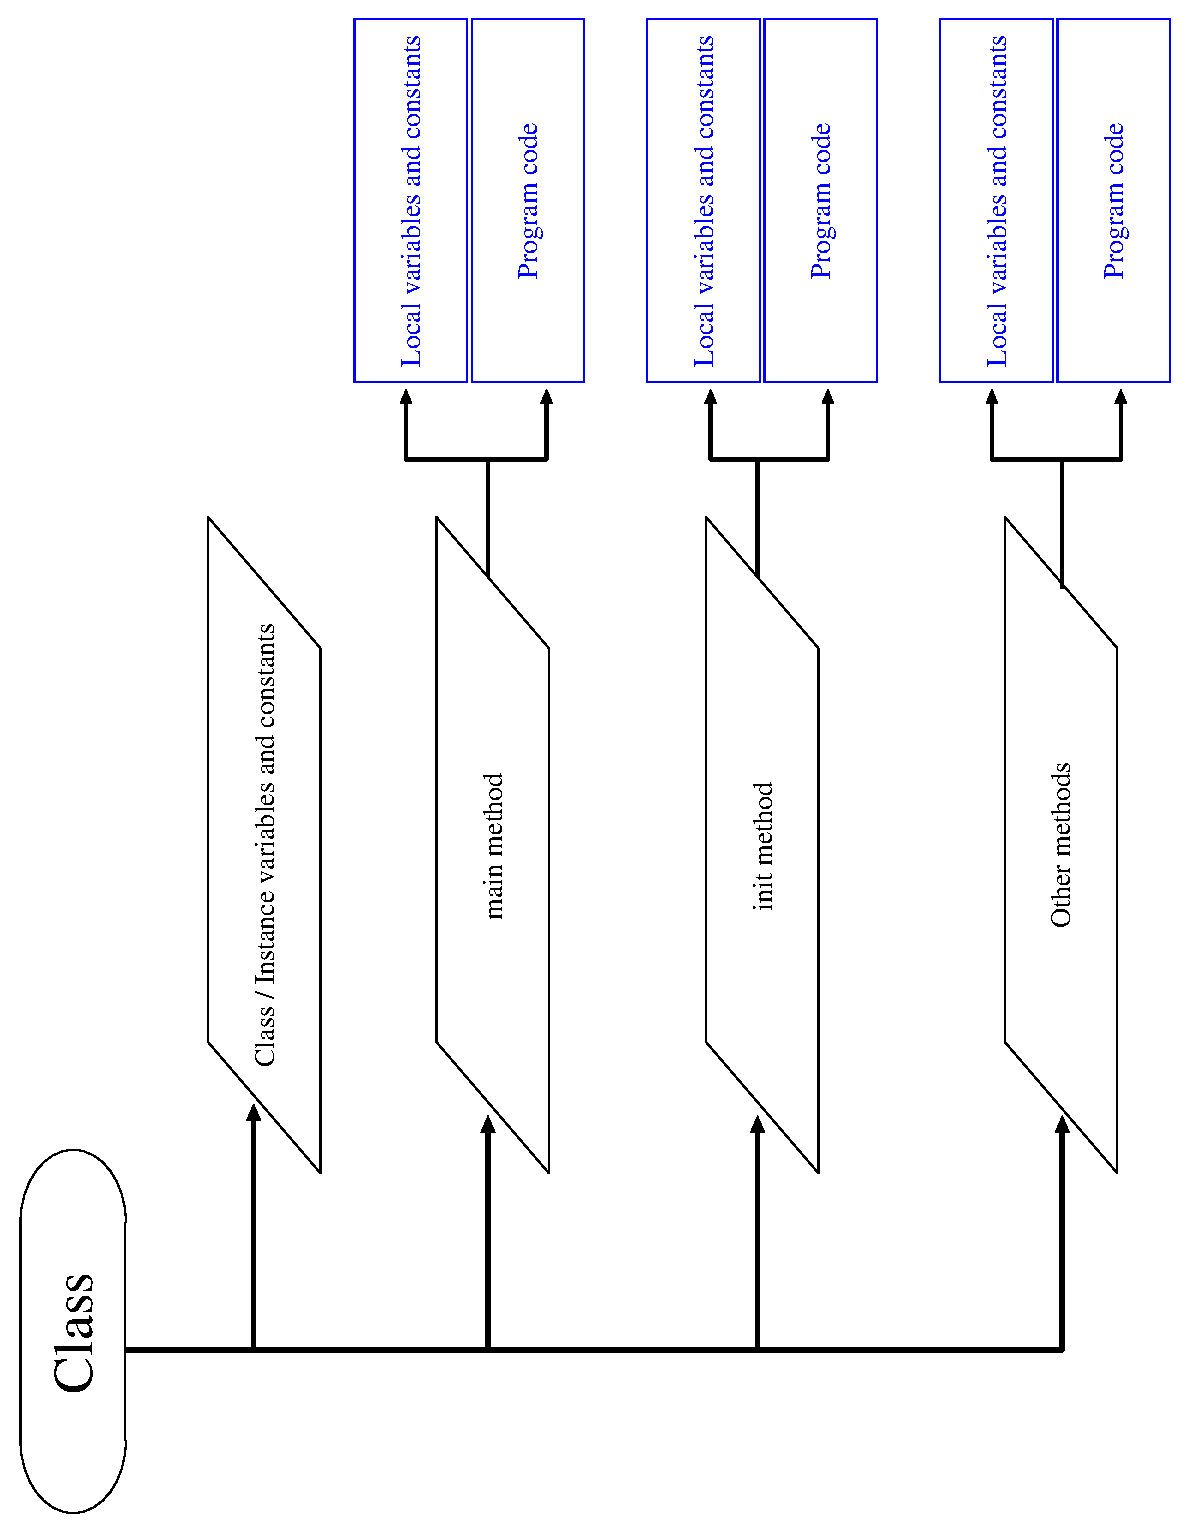
\includegraphics[angle=-90,width=\textwidth]{Figures/ClassStructure.eps}
 \caption{The class structure of a Java program, either application or an applet.}
 \label{fig:ClassStructure}
  \end{center}
\end{figure}

\section{Mathematics}
\subsection{The Java Math class}
\subsection{JNL}
\subsection{JavaSci}
\subsection{Others}
\label{sec:Others}
\section{Random Numbers}
\section{Keyboard input and Screen Output}
\section{File I/O}
\section{Ptplot}
\section{AWT}
\section{Conversions and Casting}
\section{Threads}
\section{Printing}
\section{Modifiers}
\section{Debugger}
\section{JDE and Emacs}

%%% Local Variables: 
%%% mode: latex
%%% TeX-master: "V_98"
%%% End: 
